\chapter{Konzept}

\section{Beschreibung des Fallstudien-Szenarios}
Wie in Abschnitt 2.2 erläutert, wird die Lambda-Architektur besonders häufig in Smart City-Anwendungen eingesetzt, da diese Systeme eine kontinuierliche Verarbeitung großer Sensordatenmengen erfordern. Diese Erkenntnis aus der Literatur hat uns dazu inspiriert, ein Szenario aus einem ähnlichen Bereich zu wählen, das die Anforderungen an eine Lambda-Architektur erfüllt. Wir haben uns für die Analyse von Parkhäusern entschieden, da hier eine Kombination aus Echtzeit- und Langzeitanalyse erforderlich ist, um wertvolle Erkenntnisse zu gewinnen.

Ziel unserer Fallstudie ist es, eine reale Anwendungssituation zu simulieren, in der es sinnvoll ist, die Lambda-Architektur zur Datenverarbeitung und -analyse einzusetzen. Unser Szenario basiert auf einem Parkhaus, das an den Ein- und Ausfahrten mit Kameras ausgestattet ist. Diese Kameras erfassen ein- und ausfahrende Fahrzeuge, deren Kennzeichen und Fahrzeugmerkmale gespeichert werden. Zusätzlich werden Zeitstempel der Ein- und Ausfahrten erfasst (Siehe Abbildung 3.1).

\begin{figure}[h] % [h] bedeutet "here" (hier)
    \centering
    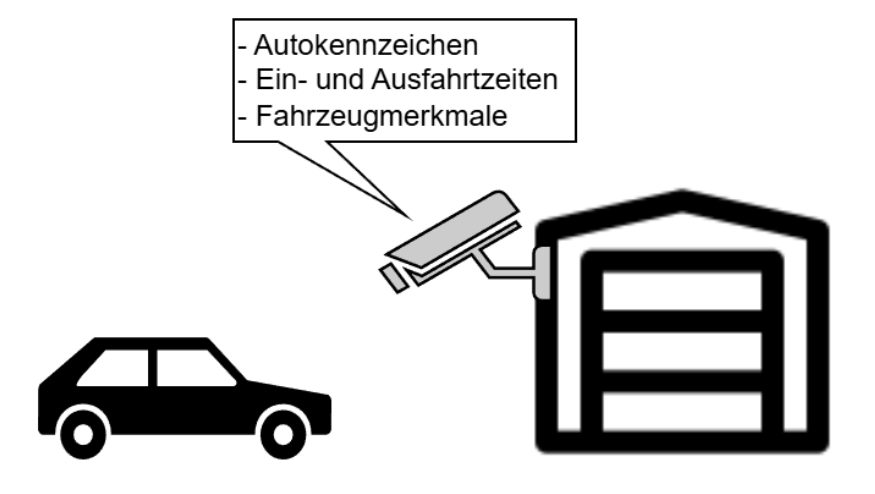
\includegraphics[width=0.8\textwidth]{Graphics/Parkhaus.png} % Bild einfügen
    \caption{Aufbau der Lambda-Architektur \cite{entwickler_lambda_kappa}.}
    \label{fig:beispielbild}
\end{figure}

Die gesammelten Sensordaten können für zwei verschiedene Arten von Analysen verwendet werden. Zum einen ermöglicht die Langzeitanalyse die Untersuchung von Spitzenzeiten, typischen Auslastungsmustern und Trends über mehrere Wochen oder Monate.  Zum anderen erlaubt die Echtzeitanalyse die Berechnung der aktuellen Anzahl geparkter Fahrzeuge.

Um sicherzustellen, dass unser Szenario tatsächlich eine große Menge an Sensordaten verarbeiten kann, erweitern wir die Fallstudie auf mehrere Parkhäuser, die zentral verwaltet werden. Dies stellt eine zusätzliche Herausforderung an die Architektur dar, da nun nicht nur die Daten eines einzelnen Parkhauses verarbeitet werden müssen, sondern die Datenströme mehrerer Standorte in einem verteilten System aggregiert und analysiert werden (Siehe Abbildung 3.2).

\begin{figure}[h] % [h] bedeutet "here" (hier)
    \centering
    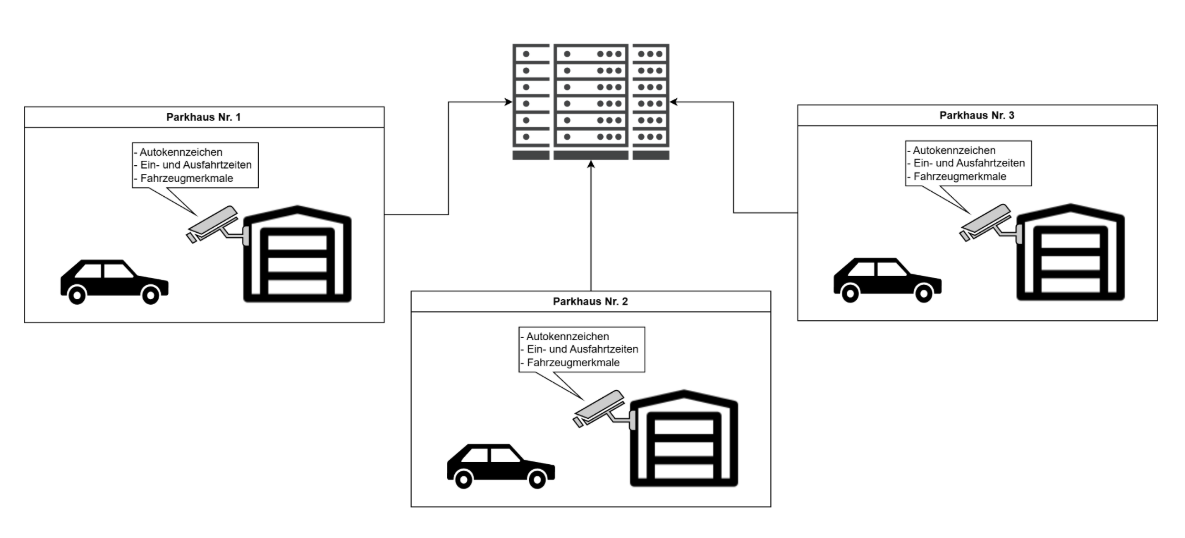
\includegraphics[width=0.8\textwidth]{Graphics/Parkhaus2.png} % Bild einfügen
    \caption{Aufbau der Lambda-Architektur \cite{entwickler_lambda_kappa}.}
    \label{fig:beispielbild}
\end{figure}

Da wir in unserer Fallstudie keine realen Kameras zur Datenerfassung verwenden können, werden wir einen Sensordatengenerator entwickeln, der realistische Ein- und Ausfahrtsereignisse simuliert. Dieser Generator wird kontinuierlich synthetische Sensordaten erzeugen, die in unser System eingespeist werden und so einen realistischen Datenfluss simulieren.

\subsection{Warum eignet sich dieses Szenario für die Lambda-Architektur?}
In Abschnitt 2.4 wurden anhand der Literatur die zentralen Eigenschaften der Lambda-Architektur identifiziert. Es wurde analysiert, welche Vor- und Nachteile diese Architektur aufweist und für welche Anwendungsfälle sie besonders geeignet ist. Aufbauend auf diesen Erkenntnissen kann begründet werden, warum das von uns gewählte Szenario optimal für die Umsetzung mit der Lambda-Architektur geeignet ist.

Ein wesentlicher Aspekt unseres Szenarios ist die zentrale Verwaltung beliebig vieler Parkhäuser, wodurch kontinuierlich große Mengen an Sensordaten erfasst und verarbeitet werden müssen. Diese Daten stammen von Kameras an den Ein- und Ausfahrten der Parkhäuser, die Informationen über ein- und ausfahrende Fahrzeuge einen zugehörigen Zeitstempel liefern. Wenn hinreichend viele Parkhäuser Daten liefern, stellt ein solcher kontinuierlicher Datenstrom hohe Anforderungen an die Datenverarbeitung. Genau für solche Szenarien wurde die Lambda-Architektur entwickelt, da sie die Verarbeitung kontinuierlich eingehender Sensordaten mit Langzeitdatenanalysen kombiniert.

Einfache Datenverarbeitung basierend auf einer Datenhistorie in einer Datenbank wäre in unserem Szenario ineffizient, da die zu verarbeitende Datenmenge mit jedem neuen Ereignis zunimmt.
Wenn beispielsweise die aktuellen Füllstände der Parkhäuser aus immer aus den in einer Datenbank hinterlegten Park-Ereignissen berechnet würden, müsste bei jeder Ein- oder Ausfahrt eines Fahrzeugs oder bei jedem Abruf des Füllstandes alle vorhandenen Daten neu analysiert werden, um die aktuelle Auslastung des Parkhauses zu berechnen.
Die Beschränkung auf den aktuellen Tag führt zu verfälschten Ergebnissen, da Autos nicht am selben Tag in ein Parkhaus Ein- und Ausfahren müssen.
Daher würden mit stetig wachsender Anzahl der Datensätze Abfragezeiten steigend und die Performance sinken.
Die Lambda-Architektur bietet hier eine Lösung durch die Kombination von Echtzeit- und Langzeitanalyse: Der Speed-Layer ermöglicht die sofortige Berechnung der aktuellen Parkhausauslastung, relativ zum letzten Batch-Füllstand, während der Batch-Layer Langzeitanalysen zu Füllhistorie, Stoßzeiten oder Nutzungsmustern liefert.

Ein weiterer wichtiger Faktor ist die Skalierbarkeit unseres Szenarios. Da unser System nicht auf ein einzelnes Parkhaus beschränkt ist, sondern potenziell viele Standorte verwalten kann, müssen neue Datenquellen problemlos integriert werden können. In einer herkömmlichen Architektur würde die Integration zusätzlicher Sensordaten zu einem erhöhten administrativen und technischen Aufwand führen. Im Gegensatz dazu wurde die Lambda-Architektur speziell für hochskalierbare verteilte Systeme entwickelt, so dass neue Parkhäuser und Sensordatenquellen dynamisch hinzugefügt werden können, ohne die bestehende Architektur wesentlich zu verändern. Die Skalierbarkeit wird durch den Einsatz verteilter Technologien gewährleistet.

Darüber hinaus spielt die Fehlertoleranz in unserem Szenario eine zentrale Rolle. Sensordaten sind fehleranfällig, sei es durch technische Defekte der Kameras oder durch unvollständige Erfassung der Fahrzeuge. Die Lambda-Architektur bietet mit ihrem Konzept der Immutable Data eine Lösung:
Da alle Rohdaten beibehalten werden, können fehlerhafte oder unvollständige Daten nachträglich korrigiert werden, sofern die für eine Korrektur notwendigen Informationen zur Verfügung stehen, wie beispielsweise im Falle einer falsch kalibrierten Waage.
Nach der Korrektur können das Batch-Layer basierend auf den korrigierten Rohdaten nochmal alle sich daraus ergebenden Daten berechnen.
